\classheader{2018-06-30}
\subsection*{Bifurcations}
Consider the autonomous $y' = f(a,y)$ where "a" is a parameter. (an uniform constant). Equilibrium may depend on the value of a (in location \# and stability type).
\begin{example-N}
	$\dot{y} = ay - y^3 = y(a-y^2)$\\
	Here, for $a < 0$, and $a > 0$, the number of equilibria are different, also the type.
	\begin{center}
		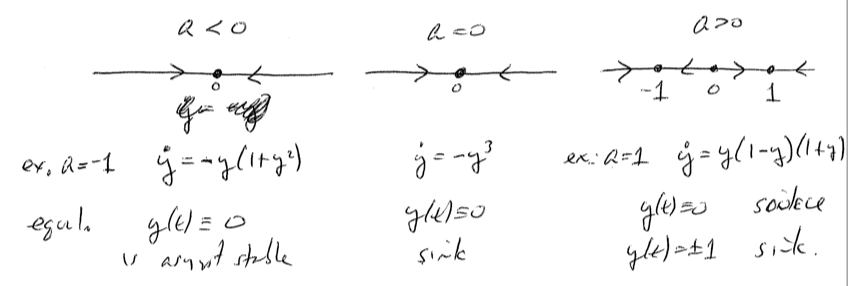
\includegraphics{7-8}
	\end{center}
\end{example-N}
We can study how $"a"$ affects equilibrium via a \underline{bifurcation diagram}
\begin{definition-N}
	A bifurcation diagram is graph of equilibrium (and stability) in relation to parameter value.
\end{definition-N} 
\redhline\\\\
{\large \underline{\textbf{Properties}}}
\begin{center}
	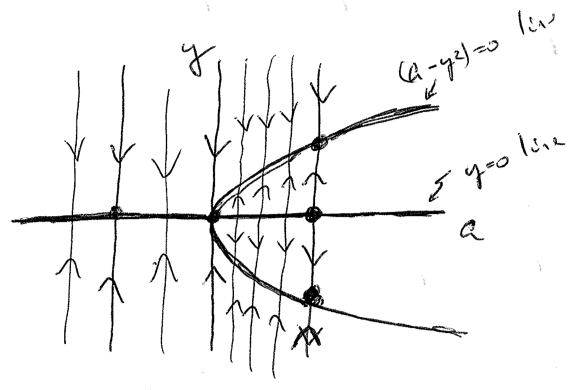
\includegraphics{7-9}
\end{center}
\begin{itemize}
	\item Each vertical slice is the phase line for a value of $a$.
	\item As $a$ varies, equilibrium trace out curves of fixed points. Found by solving $f(a,y) = 0$
	\item Curves of fixed points can be found by solving $f(a,y) = 0$\\
	$f(a,y) = y(a-y^2) = 0$, \quad when $\underbrace{y = 0}_{\text{a-axis}} \quad \underbrace{y^2 = a}_{\text{sideways parabola}} \Rightarrow y = \sqrt{a},$  $y = -\sqrt{a}$
	\item Here the only bifurcation value is $a = 0$
	\item Values of $a$ in which the stability and or \# of equilibria change are called \underline{bifurcation values} of $a$.
	\item \boxed{\text{These are rare!}} - stability cannot change outside of these!
\end{itemize}
{\Large \underline{Notes}}
\begin{enumerate}[label=\protect\circled{\Roman*}]
	\item Stable lines are used as phase lines to denote stability.
	\item Stability cannot change outside of bifurcation points, and cannot change far away.
	\item $a=0$ is called a pitchfork bifurcation for $\dot{y} = ay-y^3$.
\end{enumerate}
\begin{example-N}
	$\dot{y} = a-y^2$
	\begin{center}
		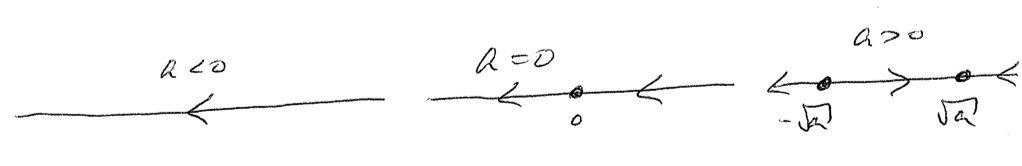
\includegraphics{7-10}
	\end{center}
	Lines of equil can only be $a-y^2 = 0 \Rightarrow a=y^2$ (sideways par).
	\begin{center}
		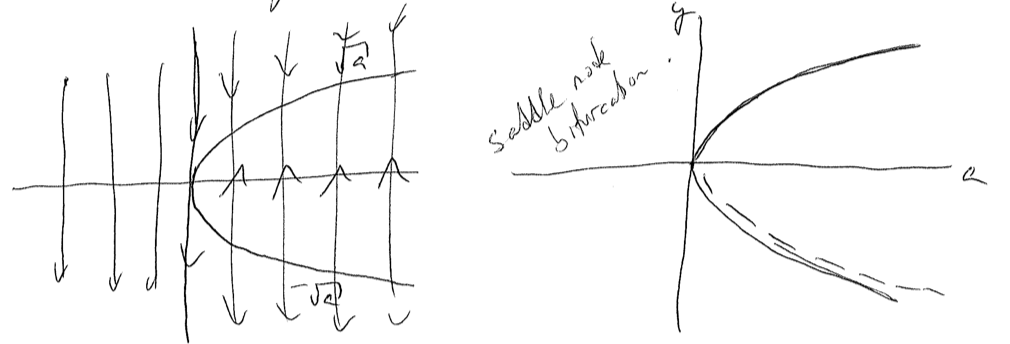
\includegraphics{7-11}
	\end{center}
\end{example-N}
\begin{example-N}
	$\dot{n} = (GN_0 - k)n - Gn^2$\\
	is an equation involving laser physics where $G, N_0, k$ are positive constants. $n(t)$ is the \# of photons along (always $n \geq 0$).\\
	Equilibrium solutions are $n(GN_0 - k - Gn) = 0$, where $n = 0$, $n = N_0 - \frac{k}{a}$.
	\begin{center}
	\underline{Bifurcation diagram.}\\
		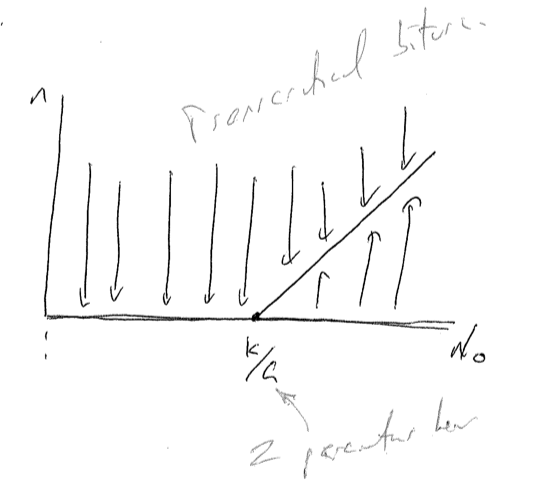
\includegraphics[scale=0.8]{7-12}
	\end{center}
\end{example-N}
\begin{enumerate}[label=\protect\circled{\Roman*}]
	\item when $N_0 < \frac{k}{a}$\\
	$\Rightarrow GN_0 - k < 0$\\
	$\Rightarrow \dot{n} < 0$\\
	$\Rightarrow n = 0$ is sink
	\item When $N_0 > \frac{k}{a}$, $GN_0 - k > 0$\\
	$\Rightarrow GN_0 - k - Gn$\\
	$N_0 - \frac{k}{a} - n > 0$ for small $n$.\\
	$\Rightarrow n = 0$ is a source\\
	if $N_0 - \frac{k}{a} - n < 0$ for $n > N_0 - \frac{k}{a}$\\
	$\Rightarrow N_0 - \frac{k}{a}$ is a sink
\end{enumerate}
\redhline\\
{\large \underline{Change track}} - Recall for any equation involving $x,y$,
\begin{itemize}
	\item We can bring all terms to one side of the equation and create an equivalent equation $\varphi (x, y) = 0$. For $\varphi (x,y)$ a function of 2 variables. Then the \underline{curve} in the xy-plane satisfying this equation is called the 0-level set of $\varphi$.
	\begin{example}
		$y^2 = 1-x^2$. We view this equation as the 0-level set of the function $\varphi(x,y) = x^2 + y^2 - 1 = 0$
	\end{example}
	\item We can view $y$ as a implicit function of $x$.\\
	In either case, the graph of the original equation (or the $\varphi(x,y) = 0$) is a curve in $xy$-plane that in general will not look like a function.\\
	We can calculate the tangent lines to this graph via differentiation in either interpretation.
	\begin{example}
		\begin{center}
			$x^2 + xy^2 = 4$, or $\varphi (x,y) = 0$, $\varphi (x,y) = x^2 + xy^2 - 4$
		\end{center}
		\begin{equation*}
			\text{\underline{Implicit diff}}\quad \dfrac{d}{dx}(x^2 +xy^2 = 4) \Rightarrow \underbrace{2x + y^2 +2xy \dfrac{dy}{dx}} = 0
		\end{equation*}	
		\begin{equation*}
			\text{\underline{Calc III}} \quad \dfrac{d \varphi}{dx}(x,y) = \dfrac{d \varphi}{dx} + \dfrac{d \varphi}{dy} \cdot \dfrac{dy}{dx} = \underbrace{\dfrac{d \varphi}{dx} + \dfrac{d \varphi}{dy} \cdot y'}_{(\star)}
		\end{equation*}
			{\tiny when we think of y as an implicit fraction of x.}
	\end{example}
\end{itemize}